\documentclass[12pt]{article}
\usepackage{amssymb,amsmath,cite,caption,geometry,graphicx,url,hyperref,cleveref}
\addtolength{\textheight}{.8in}
\addtolength{\textwidth}{.9in}
\addtolength{\topmargin}{-.4in}
\addtolength{\evensidemargin}{-.45in}
\addtolength{\oddsidemargin}{-.45in}

\catcode`\@=11

%       This causes equations to be numbered by section

\@addtoreset{equation}{section}
\def\theequation{\arabic{section}.\arabic{equation}}

%       reset section commands

\catcode`\@=11
\def\thesection{\arabic{section}.}
\def\thesubsection{\arabic{subsection}.}
\def\thesubsubsection{\arabic{subsubsection}.}
\def\appendix{\setcounter{section}{0}
        \def\thesection{Appendix.}
        \def\theequation{\Alph{section}.\arabic{equation}}}
\def\section{\@startsection{section}{1}{\z@}{3.5ex plus 1ex minus
   .2ex}{2.3ex plus .2ex}{\large\bf}}

%      reset footnotes

\renewcommand{\thefootnote}{\fnsymbol{footnote}}
\long\def\@makefntext#1{\parindent 0cm\noindent
\hbox to 1em{\hss$^{\@thefnmark}$}#1}

% Different font in captions
\newcommand{\captionfonts}{\small}
% Attribution of images
\newcommand{\source}[1]{\caption*{Source: {#1}} }
\makeatletter  % Allow the use of @ in command names
\long\def\@makecaption#1#2{%
  \vskip\abovecaptionskip
  \sbox\@tempboxa{{\captionfonts #1: #2}}%
  \ifdim \wd\@tempboxa >\hsize
    {\captionfonts #1: #2\par}
  \else
    \hbox to\hsize{\hfil\box\@tempboxa\hfil}%
  \fi
  \vskip\belowcaptionskip}
\makeatother   % Cancel the effect of \makeatletter

\begin{document}
\begin{titlepage}
\vspace{.5in}
\begin{flushright}
June 2018\\  %date
\end{flushright}
\vspace{.3in}

\begin{center}
{\Large\bf
 Efficient Causal Dynamical Triangulations}\\  %title
\vspace{.4in}
{A.~G{\sc etchell}\footnote{\it email: acgetchell@ucdavis.edu}\\
       {\small\it Department of Physics}\\
       {\small\it University of California}\\
       {\small\it Davis, CA 95616}\\{\small\it USA}}\\[2ex]
\end{center}

\vspace{.3in}
\begin{center}
{\large\bf Abstract}
\end{center}
\vspace*{.1ex}
\begin{center}
\begin{minipage}{4.9in}
{\small
I review constructing piecewise simplicial manifolds using efficient
methods for constructing Delaunay triangulations. I then evaluate the use of
the Metropolis-Hastings algorithm in the Causal Dynamical triangulations
program. I highlight inefficiencies and propose solutions.
}
\end{minipage}
\end{center}
\end{titlepage}
\addtocounter{footnote}{-2}
\tableofcontents
\section{Introduction}

\begin{quote}
  Nevertheless, due to the inneratomic (sic) movements of electrons, atoms would have to radiate
  not only electromagnetic but also gravitational energy, if only in tiny amounts.
  As this is hardly true in nature, it appears that quantum theory would have to modify
  not only Maxwellian electrodynamics, but also the new theory of gravitation.\cite{einstein_volume_nodate}

  --Einstein, 1916 {\it Approximative Integration of the Field Equations of Gravitation, p.209}
\end{quote}

Quantum gravity is, perhaps, the preeminent hard problem\cite{steve_carlip_why_2014} remaining in theoretical physics, and has been worked on for many years\cite{rovelli_notes_2000}.

Although difficult to test experimentally, a quantum theory of gravity appears to be the key to resolving several important
questions, such as the black hole information paradox.\cite{preskill_black_1992} In many cases, the conclusions of the quantum theory reverse the results of the classical theory
(black hole complementarity\cite{almheiri_black_2013}, wormhole no-go theorems \cite{visser_lorentzian_1996}). Therefore, only a quantum theory of gravity will tell us the ultimate
fate of life, the universe, and everything (with apologies to the late Douglas Adams).\cite{adams_life_1997}

Causal Dynamical Triangulations (CDT) \cite{ambjorn_non-perturbative_2000,j._ambjorn_dynamically_2001,loll_discrete_2003,ambjorn_quantum_2013,cooperman_making_2014} is a useful
approach to quantum gravity. It is based on the Regge action\cite{regge_general_1961}, which describes General Relativity on simplicial manifolds similarly to the Einstein-Hilbert
action on differentiable manifolds, and has been independently validated in 3 and 4 dimensions.\cite{kommu_validation_2011}

Using the Metropolis-Hasting algorithm\cite{robert_metropolis-hastings_2015}, one of several Markov Chain Monte Carlo (MCMC) methods, allows
for the analysis of complex distributions in higher dimensions.\cite{grisins_metropolishastings_2014} It is also relatively straight forward to apply to calculations
of the path integral.

However, and this is the central point of this paper, Metropolis-Hastings algorithms suffer from known problems such as exponentially long convergence times to stationary
distributions and sensitivity to step size (from 23\% to 70\% is given as a suitable acceptance rate \cite{bedard_optimal_2008,xing_markov_nodate}); both may occur within the context
of CDT.

Methods such as slice sampling, Hamiltonian Monte Carlo, and simulated annealing are other methods that may be used instead, and which have comparative advantages over Metropolis
algorithms. But each has respective drawbacks:

Slice sampling \cite{neal_slice_2003} adapts to the characteristic of the sample distribution. However, it must be able to sample distributions directly, which is not always possible.
It also runs into difficulties at higher dimensions, as it is non-obvious how to obtain ``efficient" samples.

Hamiltonian Monte Carlo (HMC) computes expectations by exploring a continuous parameter space of probability distributions.\cite{betancourt_conceptual_2017}. In certain implementations
it has been shown to be extremely fast and efficient\cite{hoffman_no-u-turn_2011}, but it's not necessarily clear how to set this up for the Regge action. Additionally, the parameters
may be hard to tune, and it does not handle multimodality well, and ``crumpled" or ``polymer" phases are generic features of Monte Carlo simulations.\cite{koibuchi_phase_2004}
Nonetheless, I think this is a possibility worth exploring in a future paper.

Like HMC, simulated annealing requires a global parameter space to optimize.\cite{busetti_simulated_nodate} Implementing this in the context of CDT has not, to my knowledge,
been explored.

In this paper, I examine efficiencies in the Causal Dynamical Triangulations approach by:\\[-4ex]
\begin{enumerate}\addtolength{\itemsep}{-1.5ex}
\item Efficiently initialize using Delaunay tetrahedralization;\cite{cgal:eb-18a}  
\item Apply minimal Deterministic Finite Automata, $\epsilon$-machines from Computational Mechanics\cite{shalizi_computational_1999}, to model entropy rate and other calculations;
\item Improve the acceptance rate of Metropolis-Hastings via iteration of von Neumann's procedure
\end{enumerate}
\vspace*{-1ex}

\section{Background}

The Einstein equation describes the curvature of spacetime $R_{\mu\nu}$ in terms of the stress-energy-momentum tensor $T_{\mu\nu}$:

\begin{align}
  R_{\mu\nu}-\frac{1}{2}Rg_{\mu\nu}=8\pi G_{N}T_{\mu\nu}
\end{align}

The Riemann tensor is given by:

\begin{align}
  R_{\sigma\mu\nu}^{\rho}=\partial_{\mu}\Gamma_{\nu\sigma}^{\rho}-\partial_{\nu}\Gamma_{\mu\sigma}^{\rho}+\Gamma_{\mu\lambda}^{\rho}\Gamma_{\nu\sigma}^{\lambda}-\Gamma_{\nu\lambda}^{\rho}\Gamma_{\mu\sigma}^{\lambda}
\end{align}

Where the Affine connection $\Gamma_{\mu\nu}^{\lambda}$ is defined by:

\begin{align}
  \Gamma_{\mu\nu}^{\lambda}=\frac{1}{2}g^{\lambda\sigma}\left(\partial_{\mu}g_{\nu\sigma}+\partial_{\nu}g_{\sigma\mu}-\partial_{\sigma}g_{\mu\nu}\right)
\end{align}

And the (cylindrically symmetric) metric is:

\begin{align}
  g_{\mu\nu}=\left(\begin{array}{cccc}
    e^{2\lambda} & 0 & 0 & 0\\
    0 & -e^{2\left(\nu-\lambda\right)} & 0 & 0\\
    0 & 0 & -e^{2\left(\nu-\lambda\right)} & 0\\
    0 & 0 & 0 & -\frac{r^{2}}{e^{2\lambda}}
    \end{array}\right)
\end{align}
$R^{\rho}_{\sigma\mu\nu}$ can be thought of as encapsulating the intrinsic curvature (see \Cref{parallel-transport-figure}).
\begin{figure}
  \centering
  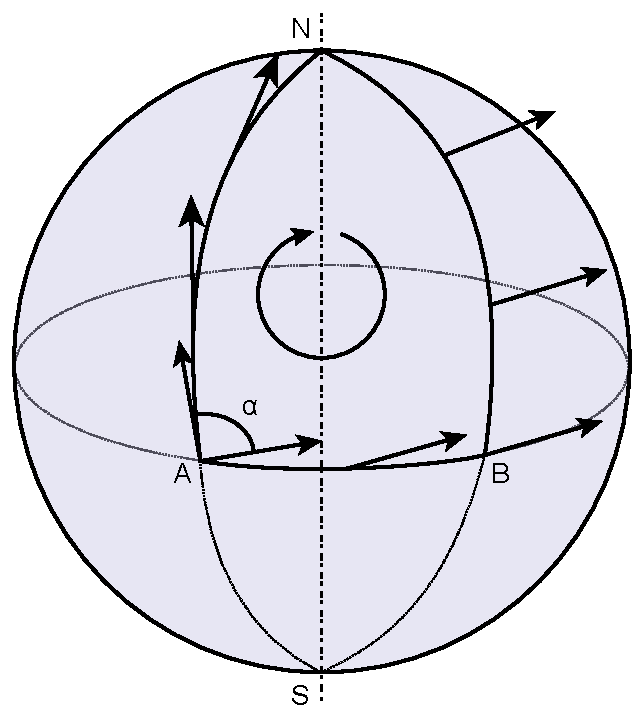
\includegraphics[width=2in]{Parallel_Transport.pdf}
  \caption{Parallel Transport on a spherical surface by Fred the Oyster, CC BY-SA 4.0, https://commons.wikimedia.org/w/index.php?curid=35124171 \label{parallel-transport-figure}}
\end{figure}

From the Riemann tensor one obtains the Ricci tensor using $R_{\mu\nu}=R^{\rho}_{\mu\rho\nu}$, and likewise the Ricci scalar is $R=R^{\mu}_{\mu}$ using the Einstein summation
convention.

Given the Ricci scalar the Einstein-Hilbert action is:

\begin{align}
I_{EH}=\frac{1}{16\pi G_{N}}\int d^{4}x\sqrt{-g}(R-2\Lambda)
\end{align}

Where $G_{N}$ is Newton's Gravitational constant and $\Lambda$ is the cosmological constant.

Extremizing the Einstein-Hilbert action produces the equations of motion.

\begin{align}
  \delta I_{EH} = 0 \rightarrow R_{\mu\nu}-\frac{1}{2}Rg_{\mu\nu}=8\pi G_{N}T_{\mu\nu}
\end{align}

In quantum mechanics, we are interested in the transition probability amplitude $\langle B|T|A\rangle$, which is the conditional probability of being in state $B$ having previously
been in state $A$. This is generally computed using the path integral.

\begin{align}
  \langle B|T|A\rangle=\int\mathcal{D}[g]e^{iI_{EH}}
\end{align}

Such path integrals are typically not directly computable, for a number of reasons. Quantum Field Theory uses perturbative summation techniques such as Feynman diagrams, but these require a notion of renormalizability for various infinite divergences, and gravity has been shown to be definitively non-renormalizable.\cite{shomer_pedagogical_2007}

In 1961 Regge developed his calculus replacing smooth differentiable manifolds with simplicial manifolds, which obey the following properties:\\[-4ex]
\begin{enumerate}\addtolength{\itemsep}{-1.5ex}
\item closed: $\forall$ $n$-dimensional simplices in the manifold each $(n-1)$-dimensional subsimplex of that simplex is also in the manifold;  
\item connected: any two $n$-dimensional simplices share at most one $(n-1)$-dimensional subsimplex;
\item geometric realization: $\exists$ a functor between the simplicial set and the category of compactly-generated Hausdorff topological spaces
\end{enumerate}
\vspace*{-1ex}

From here on, simplicial manifolds will be referred to as triangulations, as is common in the literature. (Simplicial complexes obey the first two
properties but lack a geometric realization, and may also be encountered.) Of special note are Delaunay Triangulations, which are well-behaved simplicial
manifolds with a circumspherical property of member simplices as seen in \Cref{DT}.

\begin{figure}
  \begin{center}
  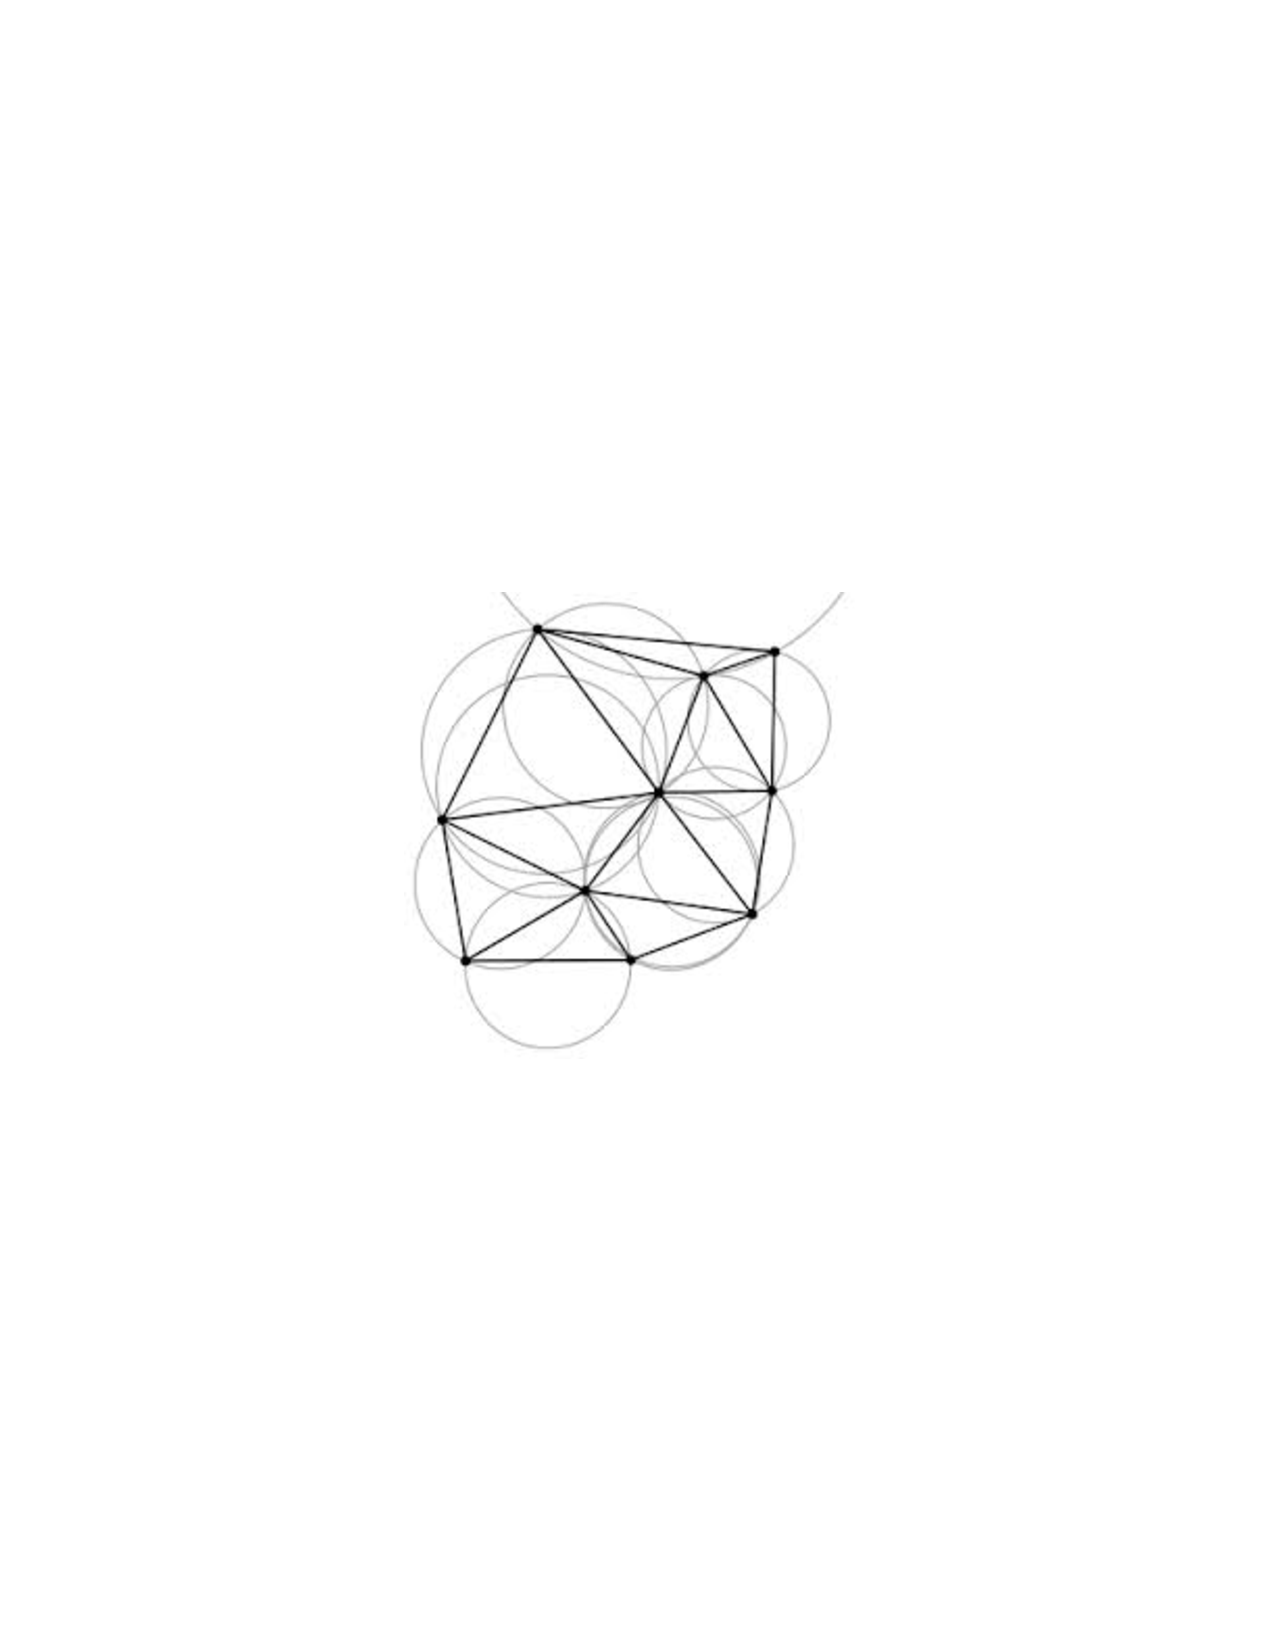
\includegraphics[width=2in]{DT1.pdf}
   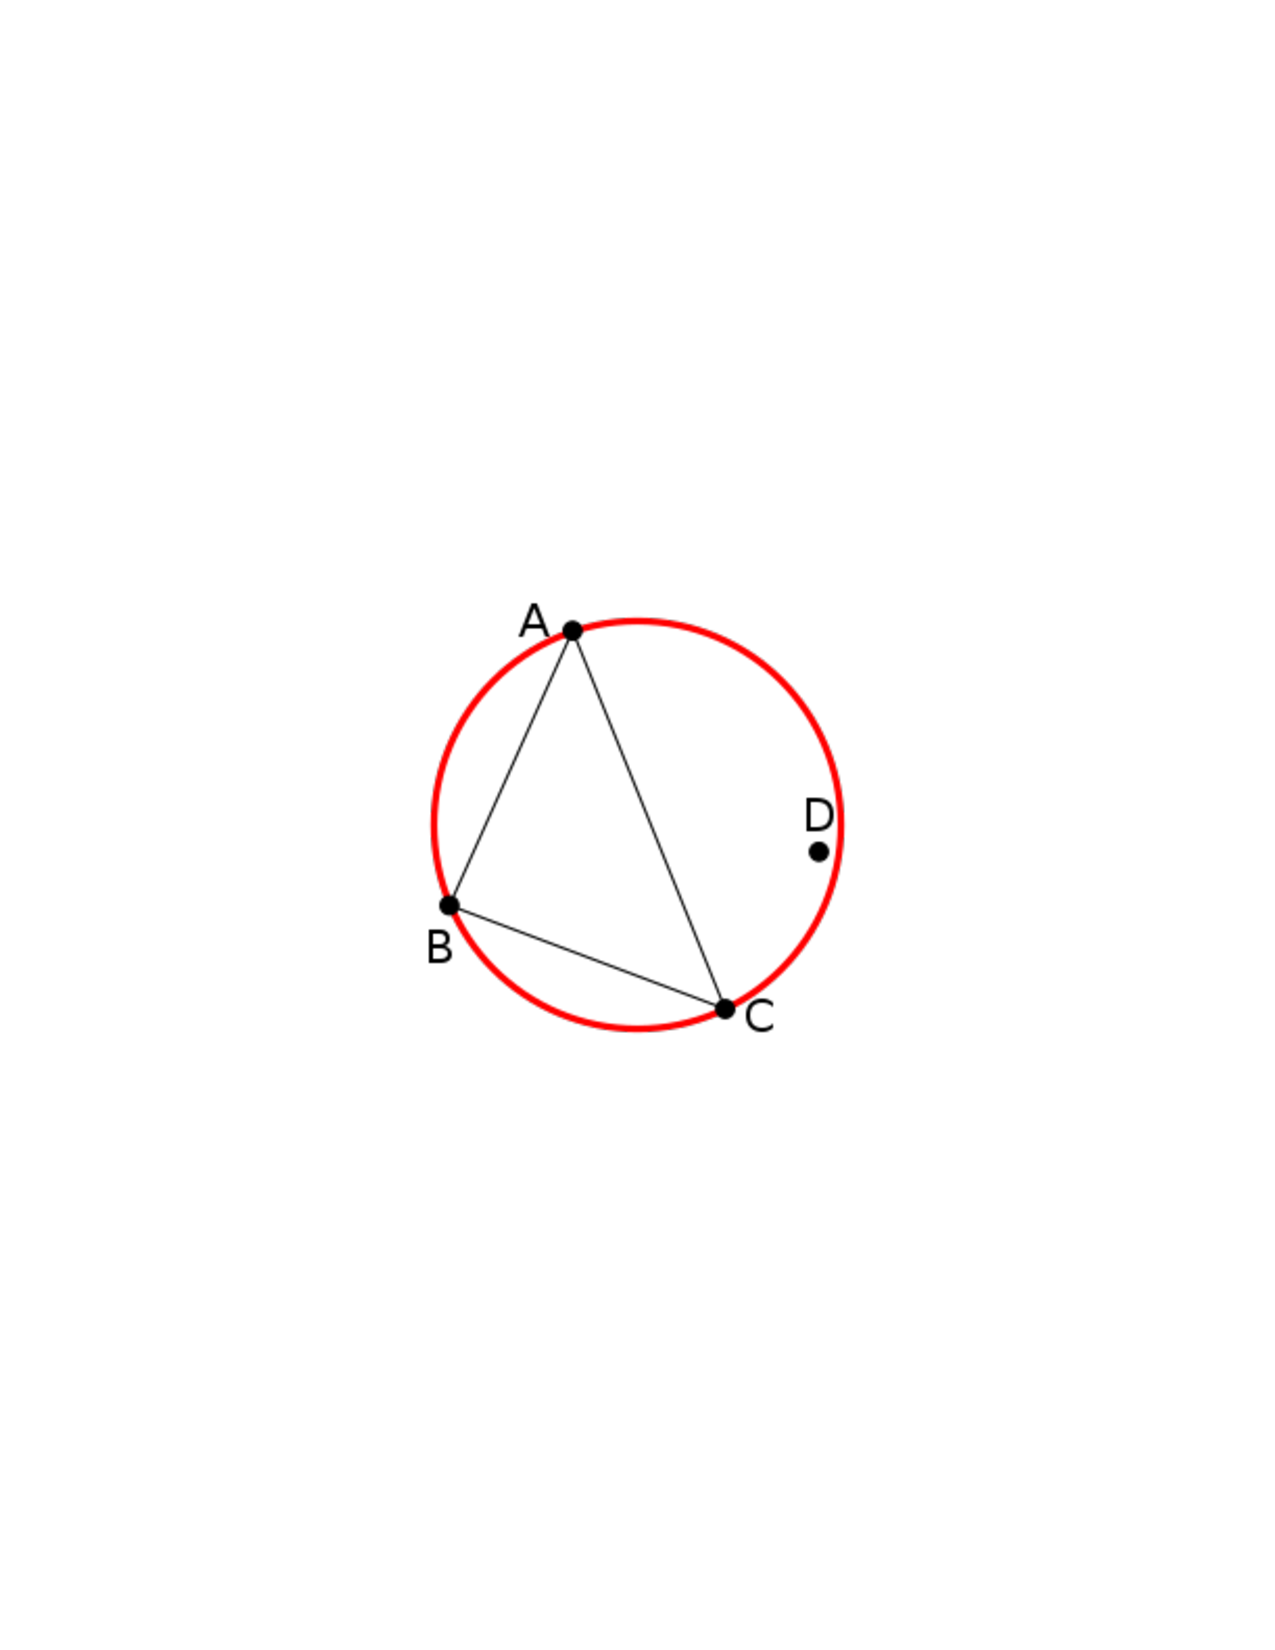
\includegraphics[width=2in]{NDT.pdf}
  \caption{A 2D Delaunay triangulation (left) Not a 2D Delaunay triangulation (right) \label{DT}}
  \end{center}
\end{figure}

The discrete version of the Einstein-Hilbert action is the Regge action:

\begin{align}
  I_{R}=\frac{1}{8\pi G_{N}}\left(\sum\limits_{hinges}A_{h}\delta_{h}-\Lambda\sum\limits_{simplices}V_{s}\right)\label{equation:Regge-Action}
\end{align}

And the discrete version of the path integral is (after a Wick rotation to imaginary time):

\begin{align}
  \langle B|T|A\rangle=\sum\limits_{triangulations\ T}\frac{1}{C(T)}e^{-I_{R}(T)} \label{CDT1}
\end{align}

Here, we take a sum over all inequivalent triangulations. In 1991 Pachner\cite{pachner_p.l._1991}, building on Alexander's work in the 1930s\cite{alexander_combinatorial_1930}
showed that elementary operations, now called Pachner moves, could transform a triangulation $T$ to another manifold $T^{\prime}$ homeomorphic to $T$. The set of all inequivalent
triangulations could be then be explored via a series of Pachner moves.\cite{gross_elementary_1992}

\Cref{CDT1} takes advantage of the distinctly causal nature of Causal Dynamical Triangulations (along with the well-defined analytic continuation). The triangulations are foliated by
hypersurfaces of distinct time. Using this innovation allows an explicit calculation of the CDT action, which has been done for 2-, 3-, and 4-dimensions. The subject of this paper is
the 3D moves (\Cref{3D-moves}) and corresponding action (Equation 35 from \cite{j._ambjorn_dynamically_2001}):

\begin{equation}
  \begin{aligned}
    I_{CDT}^{(3)} &=& 2\pi k\sqrt{\alpha}N_1^{TL} \\
    &+& N_3^{(3,1)}\left[-3k\text{arcsinh}\left(\frac{1}{\sqrt{3}
    \sqrt{4\alpha +1}}\right)-3k\sqrt{\alpha}\text{arccos}\left(\frac{2\alpha+1}
    {4\alpha+1}\right)-\frac{\lambda}{12}\sqrt{3\alpha+1}\right] \\
    &+& N_3^{(2,2)}\left[2k\text{arcsinh}\left(\frac{2\sqrt{2}\sqrt{2\alpha+1}}
    {4\alpha +1}\right)-4k\sqrt{\alpha}\text{arccos}\left(\frac{-1}{4\alpha+1}
    \right)-\frac{\lambda}{12}\sqrt{4\alpha +2}\right]\label{cdt-eq}
  \end{aligned}
\end{equation}


Where $\alpha$ is the length of the timelike edges (spacelike edges are length 1), $k=\frac{1}{8\pi G_{N}}$, and $\lambda=k*\Lambda$.

\begin{figure}
  \begin{center}
  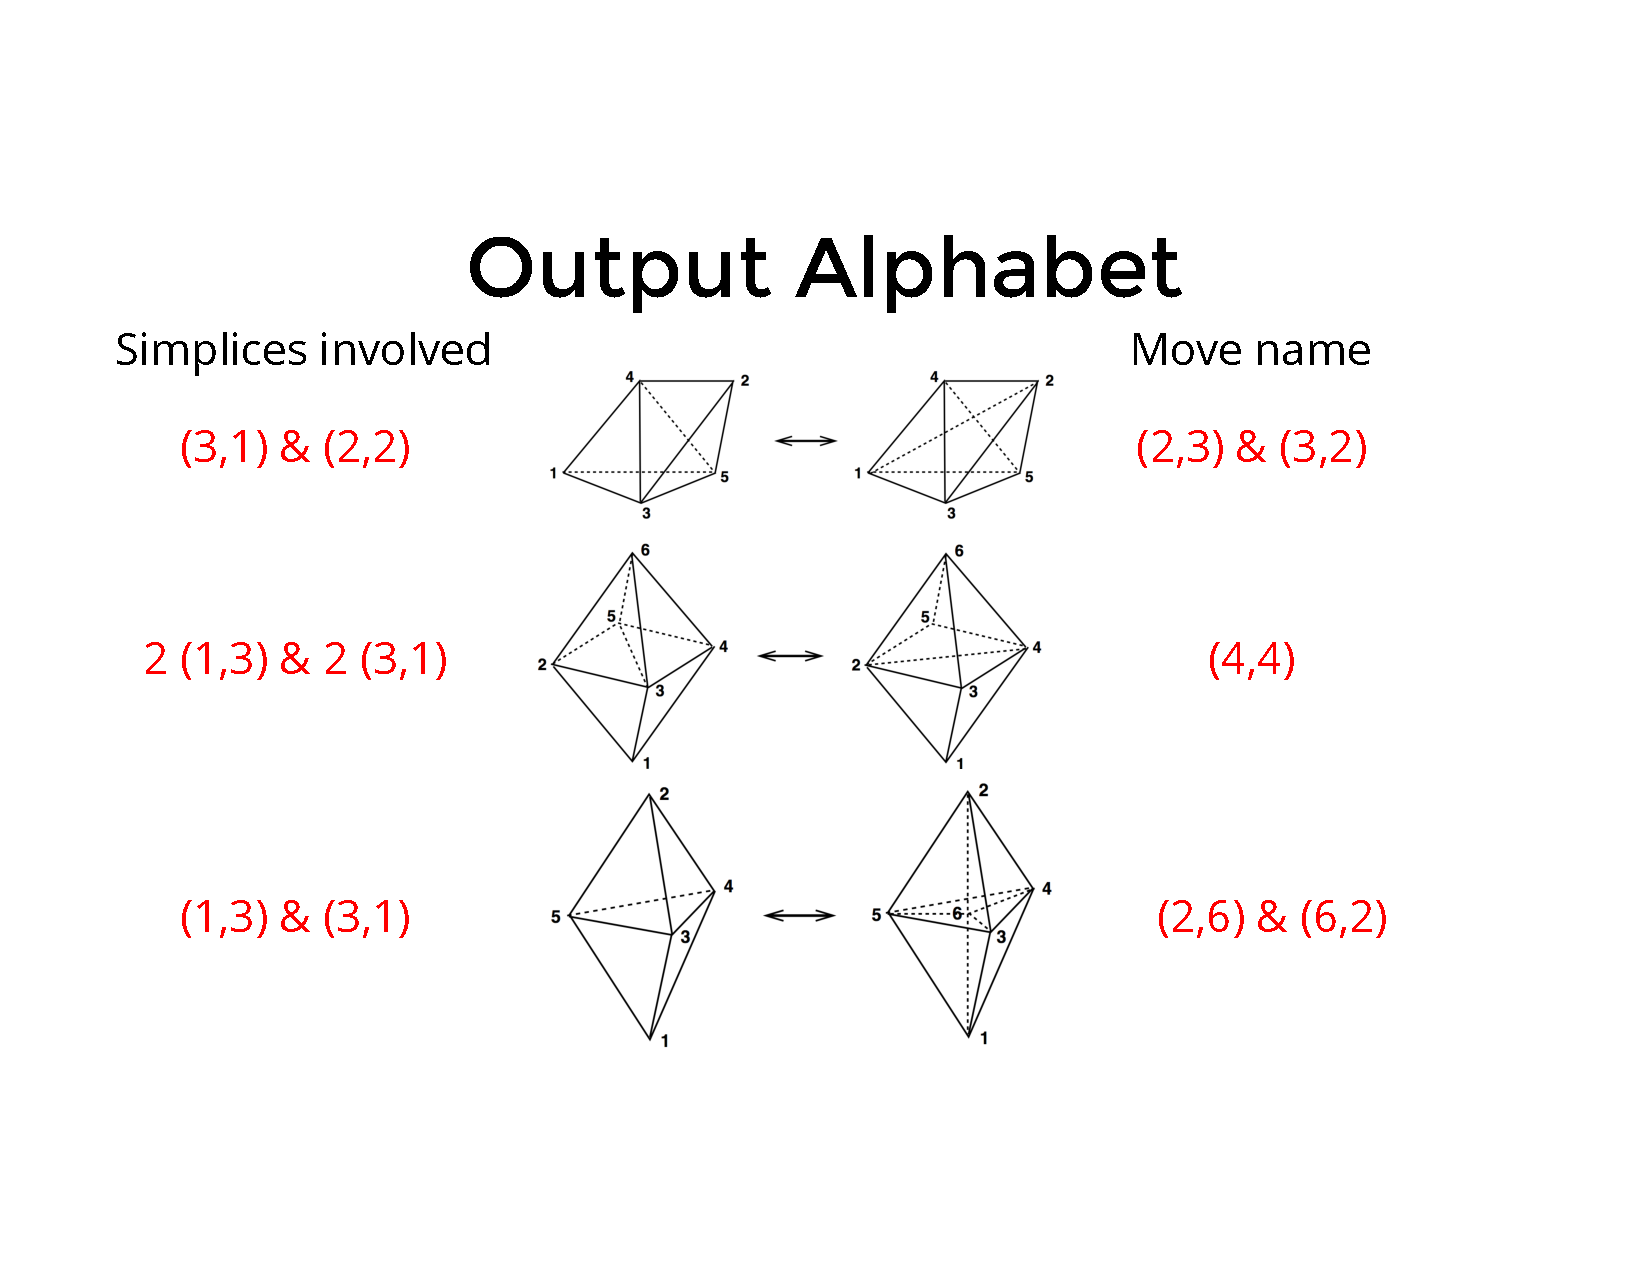
\includegraphics[width=4in]{3Dmoves.pdf}
  \caption{3D Pachner moves in CDT\label{3D-moves}}
  \end{center}
\end{figure}

To evaluate \Cref{CDT1}, we use the Metropolis-Hastings algorithm as follows:\\[-4ex]
\begin{enumerate}\addtolength{\itemsep}{-1.5ex}
\item Selection: Pick a Pachner move;  
\item Acceptance: Make that move with a probability of $a=a_1a_2$, where
\end{enumerate}
\vspace*{-1ex}

\begin{align}
  a_{1}=\frac{move[i]}{\sum\limits_{i}move[i]}
\end{align}

\begin{align}
  a_{2}=e^{\Delta I_{CDT}}
\end{align}

Note that we have divided out the measure factor $\frac{1}{C(T)}$ in \Cref{CDT1}, which we didn't know how to evaluate anyway. (It is a combinatorial weight
of the symmetry group of a particular triangulation $T$, for which we'd have to know details of the distribution we are exploring.)

After thermalization\footnote{Empirically derived at present, but another consideration for optimization.}, the Metropolis-Hastings algorithm gives us
the distribution of triangulations for computing the path integral. We can then perform measures on these representative ensembles to calculate
properties such as spectral dimension.
\cite{j._ambjorn_spectral_nodate,sotiriou_spectral_2011}

\section{Dynamical System}

A Hidden Markov Model (HMM) \cite{crutchfield_regularities_2003,singh_profile_1999} is characterized by:\\[-4ex]

\begin{itemize}\addtolength{\itemsep}{-1.5ex}
  \item[] The set of states $Q$;  
  \item[] The observables $V=\{v_k\}$;
  \item[] The initial states $\pi(i)= P(q_i|t=0)$ which is the probability of being in state $q_i$ at $t=0$.
  \item[] The transition probabilities $A=\{a_{ij}\} = P(q_j|t+1)$ which is the probability of entering state $q_j$ at $t+1$
  \item[] The observables probabilities $B=\{b_{j}(k)\} = P(v_k(t)|q_j(t))$ which is the probability of producing observable $v_k(t)$ given state $q_j(t)$.
  \end{itemize}
  \vspace*{-1ex}

  \begin{figure}
    \begin{center}
    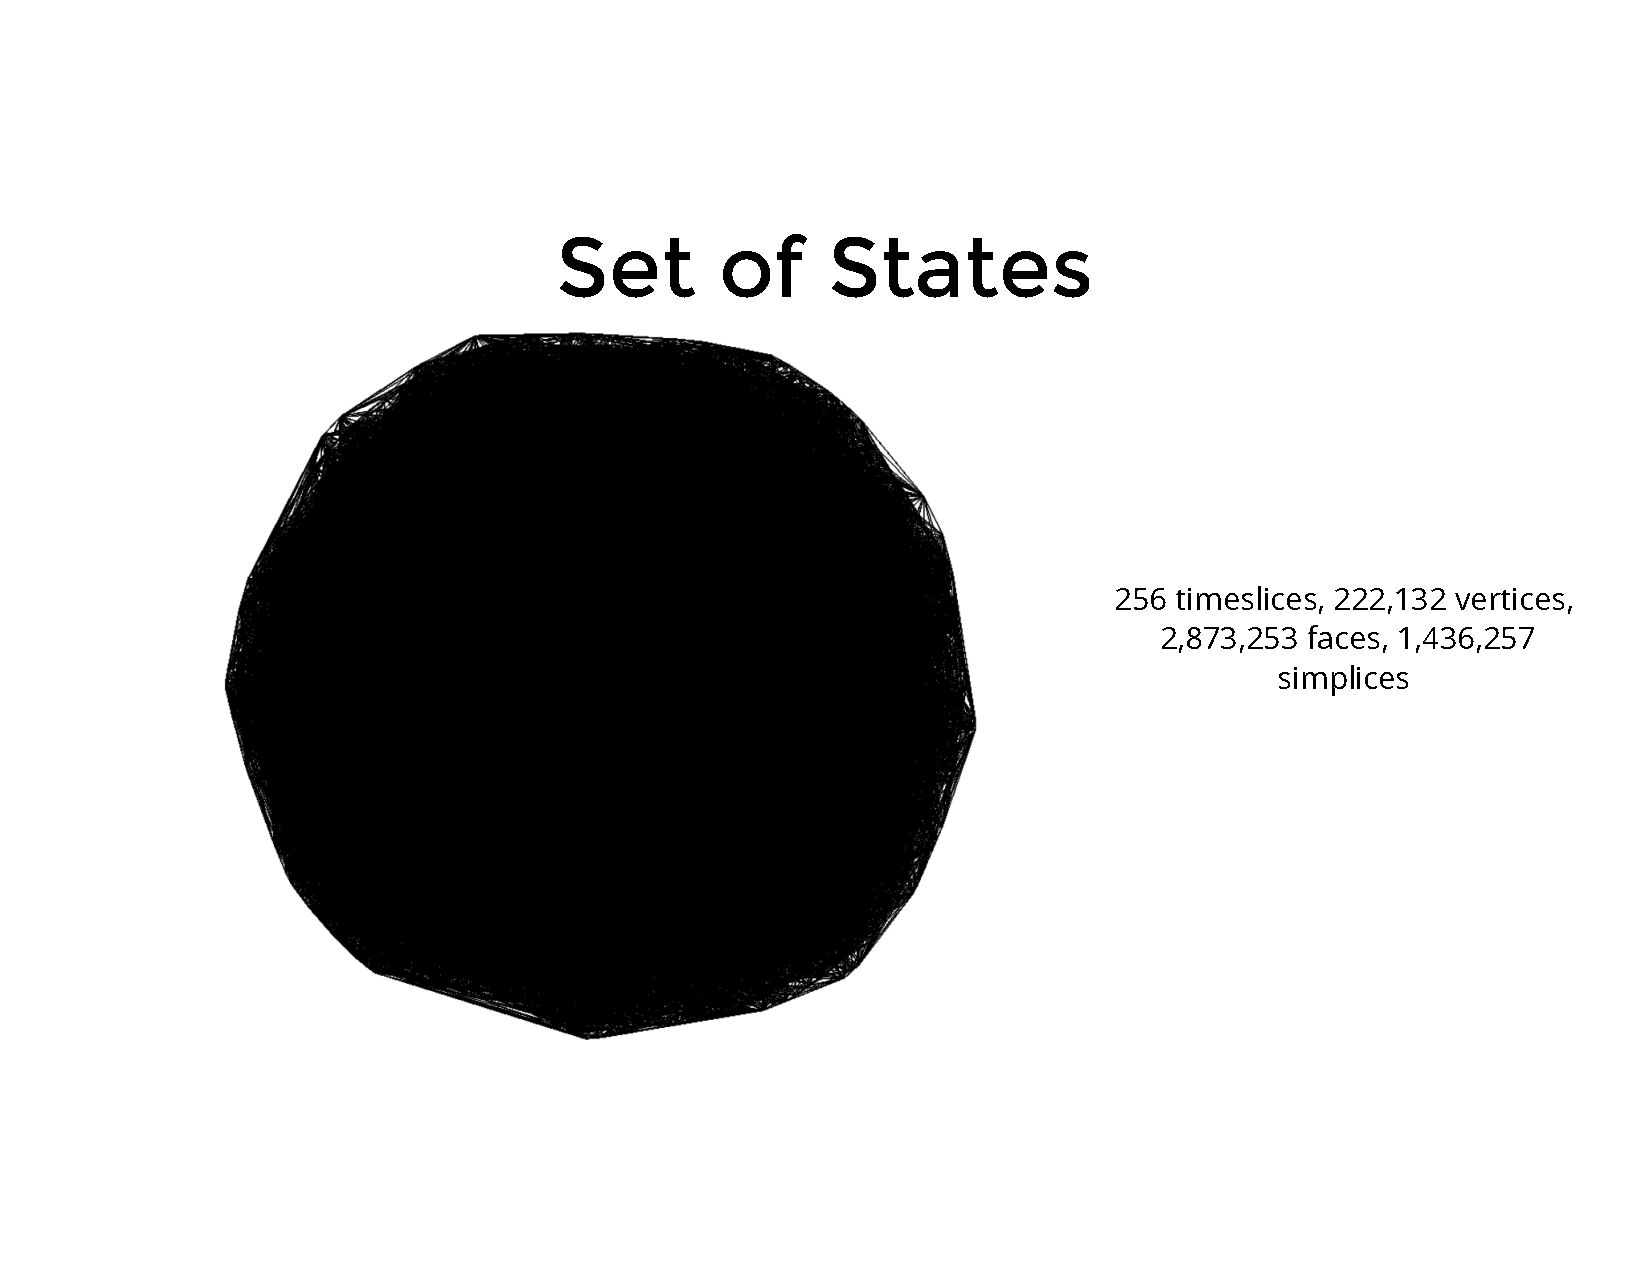
\includegraphics[width=4in]{3D-states.pdf}
    \caption{A large but representative foliated Delaunay Triangulation computed by \cite{getchell_cdt-plusplus:_2018}.\label{3D-states}}
    \end{center}
  \end{figure}

  For CDT, the states are the triangulations (\Cref{3D-states}) and the observables are the moves (\Cref{3D-moves}).

  This is an important simplification.
  
  When performing Pachner moves, the set of moves are conducted on particular simplices within the triangulation.
  A (2,3) and (3,2) move cannot be considered mutually inverse, because it is overwhelmingly likely that they will be done on different simplices;
  which then describes inequivalent triangulations.

  But from the perspective of computing \Cref{cdt-eq}, the (2,3) move is the mutual inverse of the (3,2) move, because the pair increase or decrease by one the count of simplices
  and timelike edges respectively. The same applies to the (2,6) and (6,2) moves. The (4,4) move is self-inverse and does essentially nothing, but is still distinct from
  the overwhelmingly likely no move.
  
  As we are interested in $V=\{(2,3), (3,2), (2,6), (6,2), (4,4), None\}$ this distinction preserves unifilarity in our representations of the HMM,
  and the depiction of the $\epsilon$-machine is intuitively the bi-infinite line segment.

  \begin{figure}
    \begin{center}
    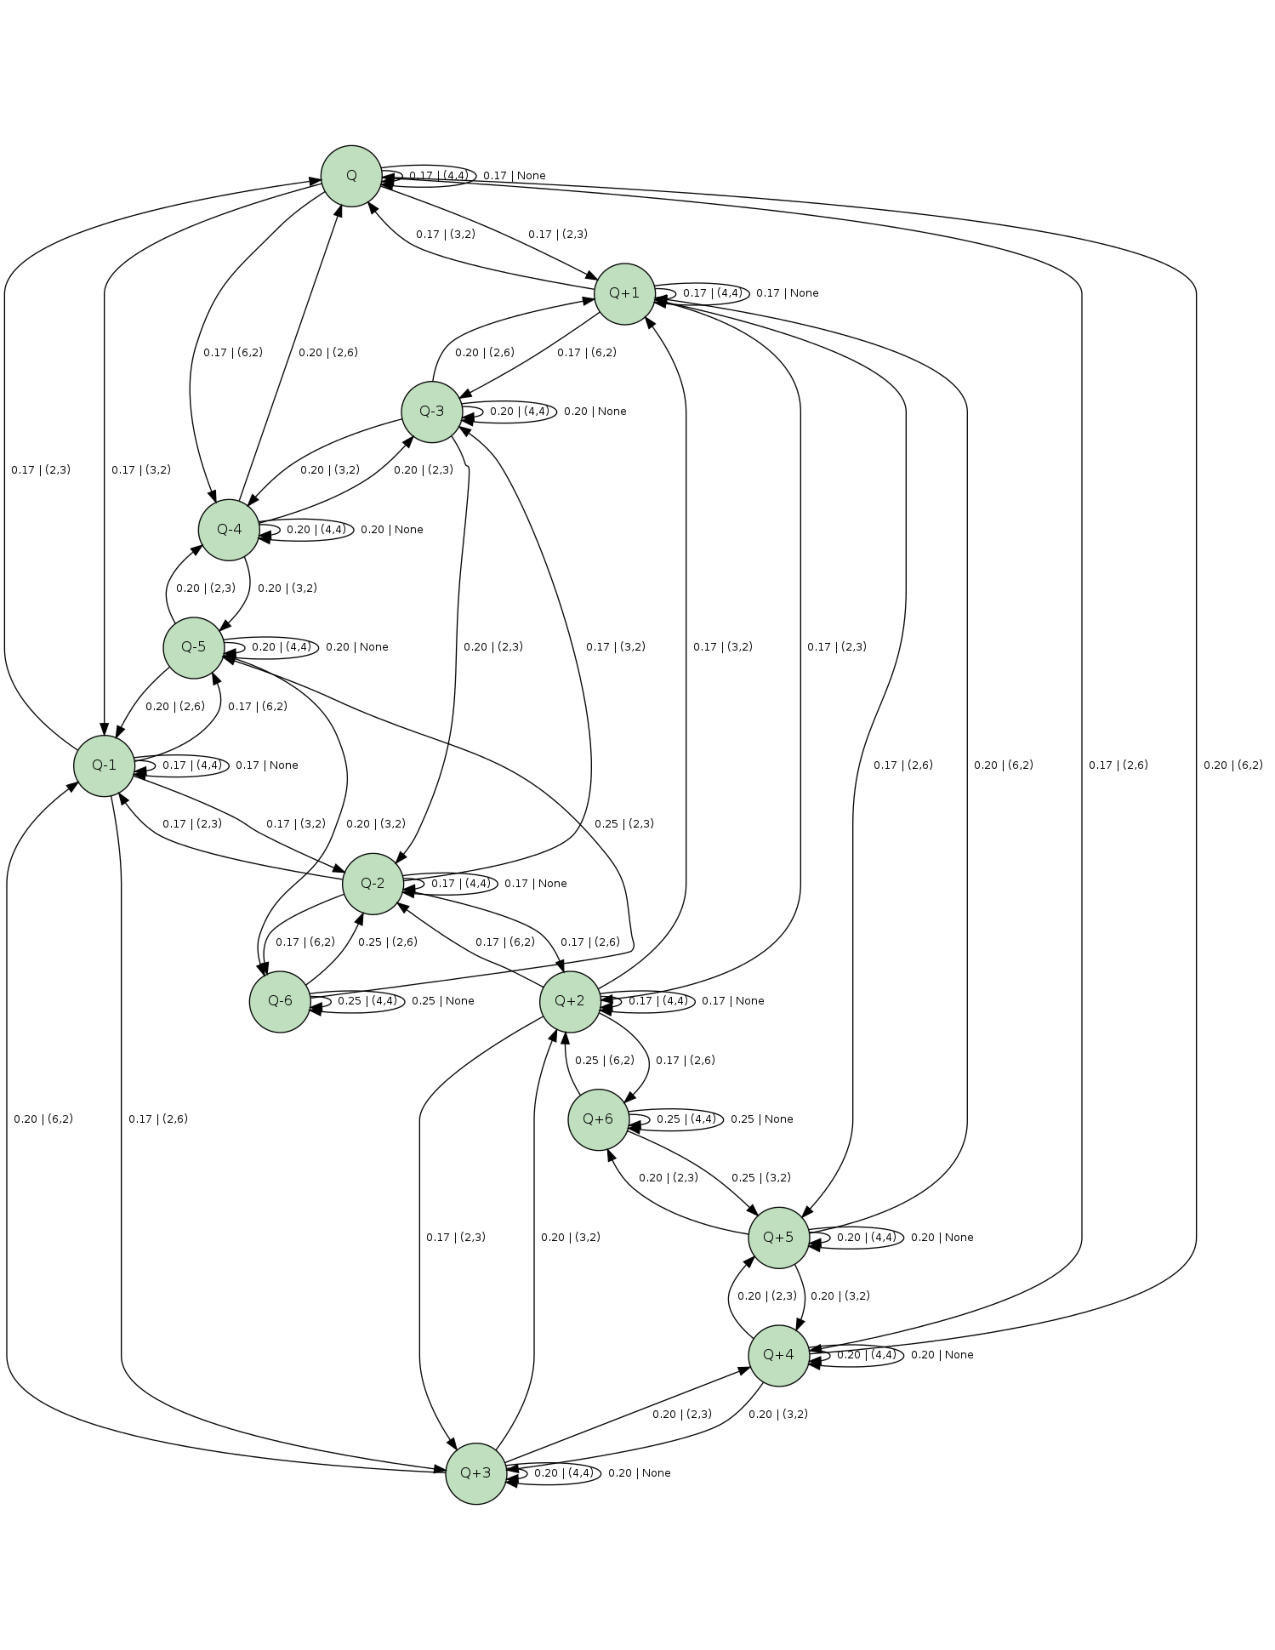
\includegraphics[width=5in]{eM-CDT.pdf}
    \caption{The $\epsilon$-machine for CDT out to a (2,6) and 2 (2,3) moves and their inverses computed on \cite{getchell_finalproject_2018}}.\label{CDT-eM}
    \end{center}
  \end{figure}

  In \Cref{CDT-eM} the states are labelled by their offset from the starting state. To unpack this diagram, let's look at the starting state $Q$, which
  is described by the following six transitions:
  
  \begin{enumerate}
    \item[] $Q\rightarrow Q+1$ emitting a (2,3) move
    \item[] $Q\rightarrow Q-1$ emitting a (3,2) move
    \item[] $Q\rightarrow Q+4$ emitting a (2,6) move
    \item[] $Q\rightarrow Q-4$ emitting a (6,2) move
    \item[] $Q\rightarrow Q$ emitting a (4,4) move
    \item[] $Q\rightarrow Q$ emitting a no-move
  \end{enumerate}

  We can likewise describe the same six (overlapping) transitions for all of the $\{Q-N,...,Q-1,Q,Q+1,Q+N\}$.
  It's easy to see that this behaves like a 1D random walk, a much simpler system than the set of Pachner moves on a 3D triangulation.

\section{Methods}

Our first method, given in the previous section, is modeling the Metropolis-Hastings algorithm with an $\epsilon$-machine to gain insight into
the particular properties of the inferred distributions from CDT.

Next, we look at more efficient algorithms in Computational Geometry, such as those provided by CGAL.

Most implementations of CDT are concerned only with the combinatorial data which specifies simplices, vertices, and the incidence and adjacency relations
between them (\Cref{combi-cell}). However, for future work that may want to impose mass or curvature and fixed distances in CDT, geometric information becomes relevant, especially for 2+1 and 3+1 spacetimes. \cite{cgal:pt-t3-18a,cgal:hdj-t-18a}

CDT implementations initialize their spacetimes by starting with a small set of cells with spherical or toroidal topology, and then making a large number
of volume-increasing and foliation preserving moves. This very regular structure is then thermalized by a very large number of additional moves (typically 50-100,000 passes, where a pass attempts a number of moves equal to the total number of simplices in the triangulation).

However, modern algorithms can directly generate 3D Delaunay triangulations very rapidly. CGAL is capable of triangulating 1 million points in about 6
seconds on a laptop, and recent algorithms have generated three billion tetrahedra in one minute on a start of the art laptop! \cite{marot_one_2018}
In my CDT implementation, I create concentric radii of points which are tetrahedralized. By marking each point with it's time value on creation,
successive sweeps are able to remove those tetrahedra that do not span two adjacent timeslices. The removed tetrahedra force a re-triangulation of the
remaining points (however, the algorithms are able to conduct this in parallel for localized regions), and the process is repeated until only validly foliated simplices remain.

The resulting triangulation is already randomized; future work will determine how much thermalization is necessary.

Further optimizations are possible.

In my implementation, prediction of the final number of simplices is difficult due to many passes which throw them away simplices. 
That is, asking for some number of simplices often produces many more than desired, and sometimes substantially less, due to seemingly random effects.

Or are they?

During this process of re-tetrahedralization, I have noticed unexpectedly divergent behavior that implies both unseen
regularities and random, possibly chaotic processes. Using parameter optimization methods from Comet.ml \cite{comet.ml_comet.ml_nodate} and
TensorFlow\cite{noauthor_tensorflow_nodate}, I have run experiments to determine optimal hyperparameters for a given output.

These experiments solve the following problem: given initial radius, radial spacing, desired timeslices, desired number of simplices, and a distribution
function of points per timeslice, what is the number of simplices obtained, and which combination of factors minimizes the difference between desired and
actual. (Related ongoing questions include developing good cost functions for optimization and good distributions).

The last method employed is von Neumann's method of improving the take rate. This essentially solves the question: how do I make an unfair coin into
a fair one? \cite{mitzenmacher_tossing_nodate} In the case of CDT, the probability of making a given move is vanishingly small: a small simulation with
16 timeslices and 490K simplices typically produces move probabilities given in \Cref{table-moveprob}. Note these are very far away from the Metropolis
ideal.

\begin{table}
\begin{center}
  \begin{tabular}{|l|l|}
    \hline
    \multicolumn{2}{|c|}{Move probabilities} \\
    \hline
    (2,3) & 0.005 \\
    (3,2) & 0.036 \\
    (2,6) & 0.031 \\
    (6,2) & 0.00200 \\
    (4,4) & 1\footnote{A (4,4) is automatically accepted to improve $A_1$}\\
    \hline
    \end{tabular}
  \end{center}
    \caption{Observed simulation values of move probabilities}
    \label{table-moveprob}
  \end{table}

Von Neumann's Procedure seems to be related to the Entropy rate. Further investigation and understanding on this point is necessary.

\begin{figure}
  \begin{center}
  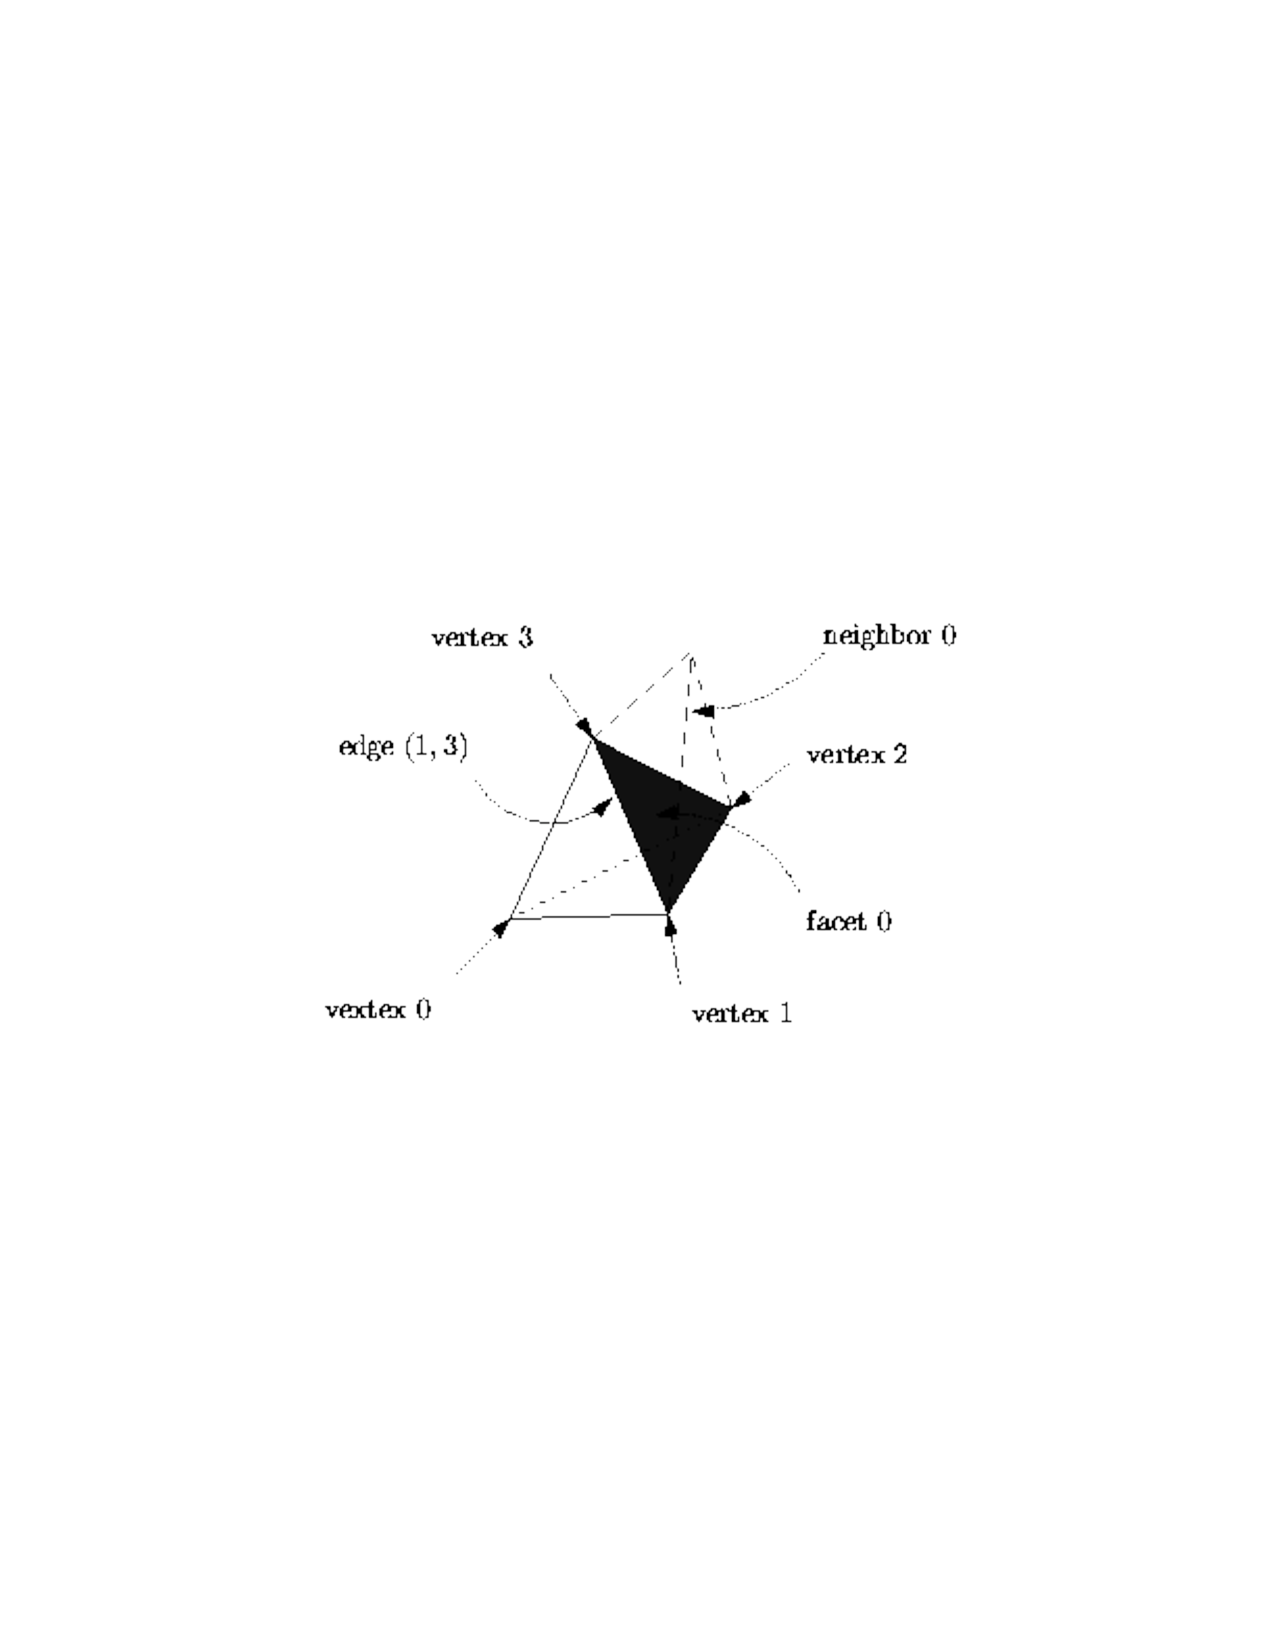
\includegraphics[width=3in]{repres.pdf}
  \caption{CGAL cell combinatorial data structure \cite{cgal:pt-tds3-18a}.\label{combi-cell}}
  \end{center}
\end{figure}

\section{Results}

For the limited $\epsilon$-machine representing the CDT HMM in \Cref{CDT-eM}, \Cref{table-cmpy} lists the calculated parameters.

The $\epsilon$-machine model itself may also be used for further simulations.

The results of hyperparameter optimization for number of simplices requested versus number obtained are available for public review at \href{https://www.comet.ml/acgetchell/cdt-plusplus}{https://www.comet.ml/acgetchell/cdt-plusplus}.

\begin{table}
  
\begin{center}
\begin{tabular}{|l|l|}
  \hline
  \multicolumn{2}{|c|}{$\epsilon$-machine Information Theoretic values} \\
  \hline
  Markov Order & $\infty$ \\
  Cryptic Order & 0 \\
  Excess Entropy & 3.68736404907 \\
  Entropy Rate & 2.40009879218 \\
  Predictive Information Rate & 2.017745851 \\
  Residual Entropy Rate &0.382352941176 \\
  \hline
  \end{tabular}
\end{center}
  \caption{Calculated values from the Computational Mechanics Python Module (CMPy) \cite{noauthor_welcome_nodate}}
  \label{table-cmpy}
\end{table}

\newpage

\section{Conclusion}

A lot of work remains to be done, but it is apparent that the principles of Computational Mechanics, Information Theory, and modern algorithms
can provide a real boost in computing efficiency over and above throwing more hardware and computer time at an admittedly intractable problem. A (perhaps
apocryphal) story related to me first hand about the race to sequence the human genome is instructive: one of the world's largest supercomputers at the
time, with custom hardware was nevertheless beaten by a plucky group of university researchers writing extremely efficient algorithms in C.\cite{nguyen_race_nodate}

I hope that time spent learning to teach computers how to calculate quantum gravity efficiently may have great impact.

\begin{figure}
  \begin{center}
  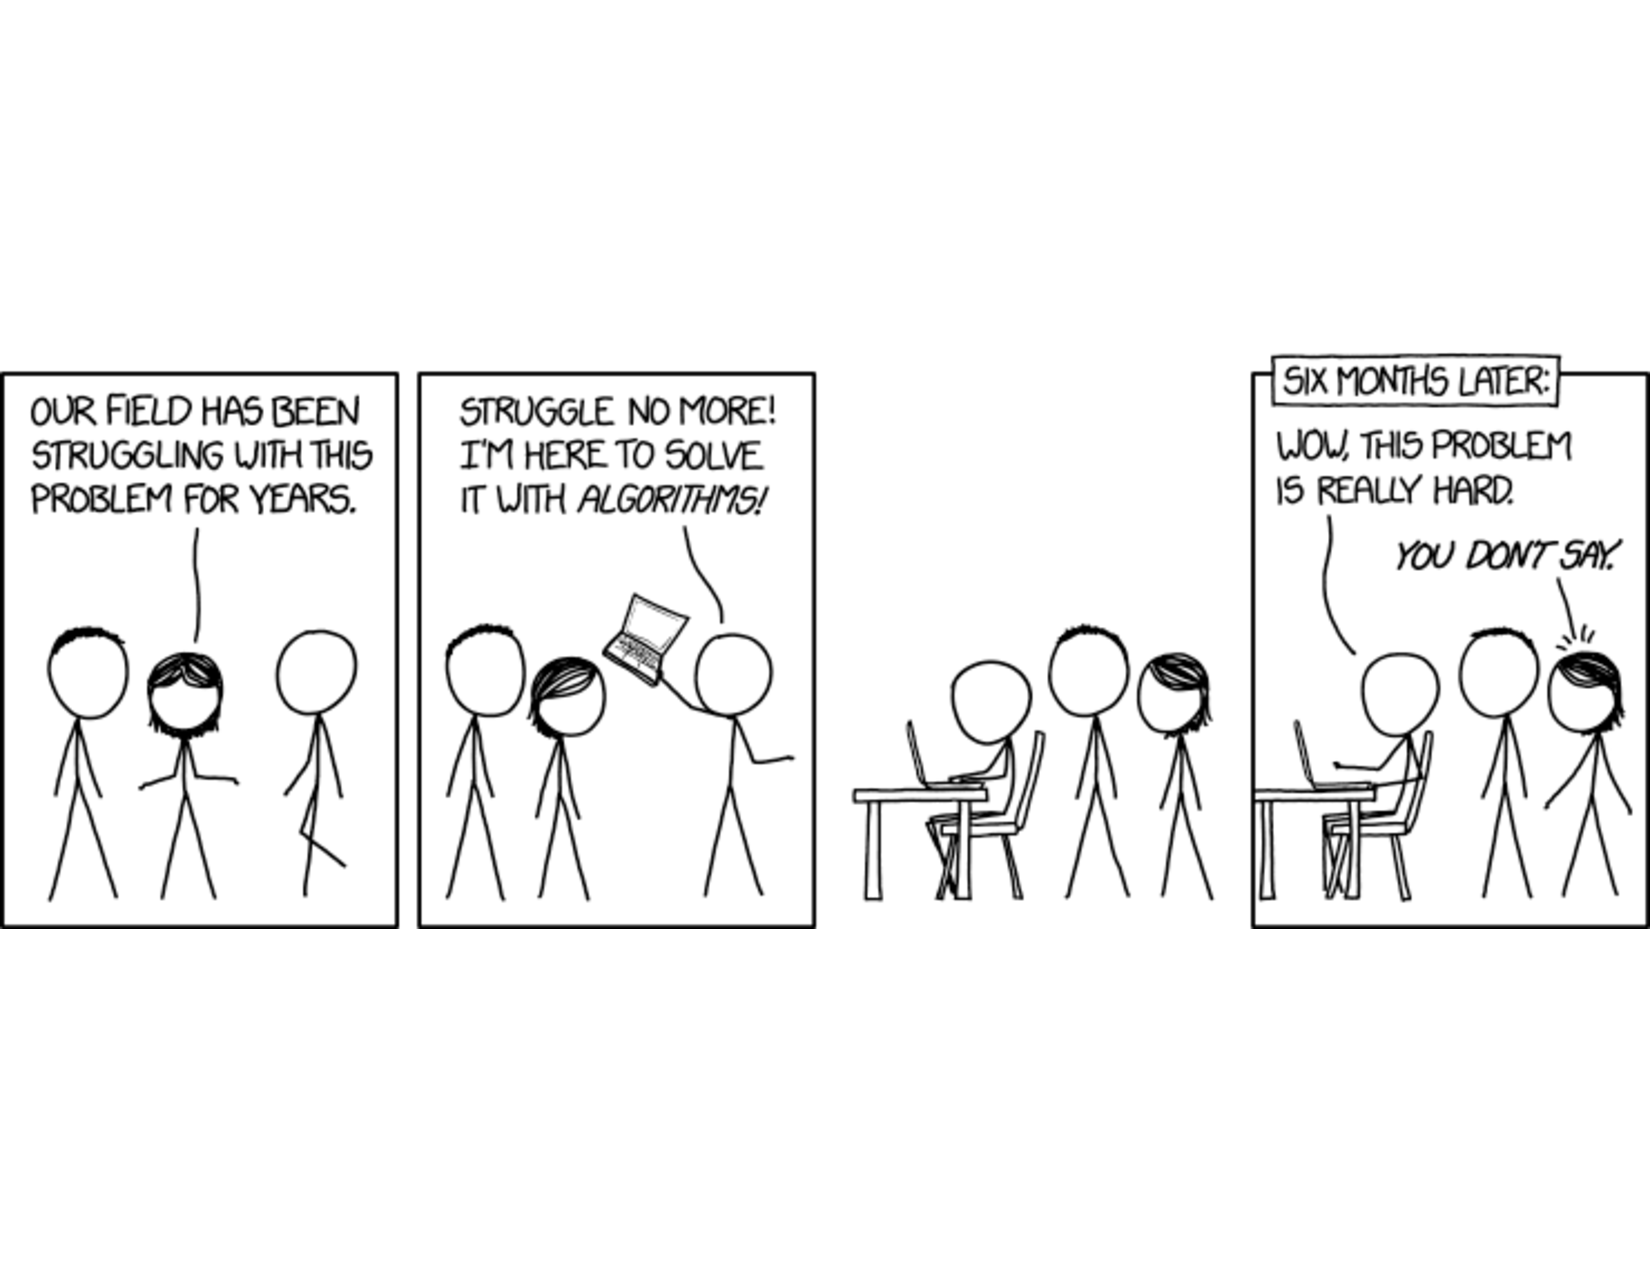
\includegraphics[width=4in]{here_to_help.pdf}
  \caption{\url{https://www.xkcd.com/1831/}}
  \end{center}
\end{figure}

\newpage

\vspace{1.5ex}

\bibliographystyle{ieeetr}
\bibliography{EfficientCDT.bib}
\end{document}
